%% 
%% Copyright 2019-2020 Elsevier Ltd
%% 
%% This file is part of the 'CAS Bundle'.
%% --------------------------------------
%% 
%% It may be distributed under the conditions of the LaTeX Project Public
%% License, either version 1.2 of this license or (at your option) any
%% later version.  The latest version of this license is in
%%    http://www.latex-project.org/lppl.txt
%% and version 1.2 or later is part of all distributions of LaTeX
%% version 1999/12/01 or later.
%% 
%% The list of all files belonging to the 'CAS Bundle' is
%% given in the file `manifest.txt'.
%% 
%% Template article for cas-dc documentclass for 
%% double column output.

%\documentclass[a4paper,fleqn,longmktitle]{cas-dc}
\documentclass[a4paper,fleqn]{cas-dc}

%\usepackage[authoryear,longnamesfirst]{natbib}
%\usepackage[authoryear]{natbib}
\usepackage[numbers]{natbib}
\usepackage{graphicx}
\usepackage{subfigure}

\begin{comment}
\def\tsc#1{\csdef{#1}{\textsc{\lowercase{#1}}\xspace}}
\tsc{WGM}
\tsc{QE}
\tsc{EP}
\tsc{PMS}
\tsc{BEC}
\tsc{DE}
%%%
\end{comment}
%%%Author definitions


\begin{document}
	\let\WriteBookmarks\relax
	\def\floatpagepagefraction{1}
	\def\textpagefraction{.001}
	\shorttitle{Survey of Multimedia Data in Manufacturing}
%	\shortauthors{Yunchao Wang et~al.}
	
	\title [mode = title]{Visualization and Visual Analysis of Multimedia Data in Manufacturing: A Survey}                      
	%\tnotemark[1,2]
	
	\begin{comment}
	\tnotetext[1]{This document is the results of the research
	project funded by the National Science Foundation.}
	
	\tnotetext[2]{The second title footnote which is a longer text matter
	to fill through the whole text width and overflow into
	another line in the footnotes area of the first page.}
	
	\end{comment}
	
	
%	\author{Yunchao Wang}
%	\author {Zihao Zhu}
%	\author{Lei Wang}
%	\author{Guodao Sun*}
%	\ead{godoor.sun@zjut.edu.cn}
%	\author{Ronghua Liang}
%	\address{College of Computer Science, Zhejiang University of Technology, Hangzhou, 310023}
	

%	\author{Guodao Sun{mycorrespondingauthor}}
%\cortext[mycorrespondingauthor]{Corresponding author}
	
	\begin{comment}
	\author[1,3]{CV Radhakrishnan}[type=editor,
	auid=000,bioid=1,
	prefix=Sir,
	role=Researcher,
	orcid=0000-0001-7511-2910]
	\cormark[1]
	\fnmark[1]
	\ead{cvr_1@tug.org.in}
	\ead[url]{www.cvr.cc, cvr@sayahna.org}
	
	\credit{Conceptualization of this study, Methodology, Software}
	
	\address[1]{Elsevier B.V., Radarweg 29, 1043 NX Amsterdam, The Netherlands}
	
	\cortext[cor1]{Corresponding author}
	
	\cortext[cor2]{Principal corresponding author}
	\fntext[fn1]{This is the first author footnote. but is common to third
	author as well.}
	\fntext[fn2]{Another author footnote, this is a very long footnote and
	it should be a really long footnote. But this footnote is not yet
	sufficiently long enough to make two lines of footnote text.}
	
	\nonumnote{This note has no numbers. In this work we demonstrate $a_b$
	the formation Y\_1 of a new type of polariton on the interface
	between a cuprous oxide slab and a polystyrene micro-sphere placed
	on the slab.
	}
	\end{comment}
	
	
	\begin{keywords}
		Visualization \sep Visual Analysis \sep Manufacturing \sep Multi-media data \sep Industry 4.0
	\end{keywords}
	
	
	\begin{abstract}
		%随着生产技术和社会需求的发展,制造业的门类不断完善。而传感器和计算机的使用,使得制造业中多媒体数据的收集越来越方便。根据多媒体数据的类型进行针对性的快速细致的分析可以在制造业全流程的不同阶段做出及时的决策。可视化与可视分析因其直观性和可交互性,在数据的理解、展示和分析上展现了强大的能力,被频繁应用在制造业多媒体数据分析中。在本文中,我们提出了一个可视化与可视分析的文献综述,专门为制造业多媒体数据。我们根据可视化技术、交互分析方法和应用领域对现有研究进行分类。在制造业研究项目的具体例子中,我们讨论了可视化和可视化分析应用于不同类型的多媒体数据时的差异。最后,我们对现有挑战做了总结,指出未来研究方向。
		With the development of production technology and social needs, sectors of manufacturing are constantly improving. The use of sensors and computers has made it increasingly convenient to collect multimedia data in manufacturing. Targeted, rapid and detailed analysis based on the type of multimedia data can make timely decisions at different stages of the entire manufacturing process. Visualization and visual analytics are frequently adopted in manufacturing multimedia data analysis because of their powerful ability to understand, present and analyze data in an intuitive and interactive way. In this paper, we present a literature review of visualization and visual analytics specifically for manufacturing multimedia data. We classify existing researches according to visualization techniques, interaction analysis methods and application areas. We discuss the differences when visualization and visual analytics are applied to different types of multimedia data in the context of specific examples from manufacturing research projects. Finally, we summarize the existing challenges and prospect the future research directions.
	\end{abstract}
	
	\maketitle
	


%  介绍
\section{Introduction}
%工业4.0的核心是智能生产技术和智能生产模式,旨在通过“物联网”和“务联网”,把产品、机器、资源和人联系在一起,推动各环节数据共享,实现产品全生命周期和全制造流程的数字化。
The core of Industry 4.0 is smart production technology and model. It aims to connect products, machines, resources and people through the \textit{Internet of Things} (IoT)~\cite{Gubbi2013} and \textit{Internet of Services} (IoS)~\cite{Cardoso2010}, promote data sharing in all aspects, and realize the digitalization of the whole product life cycle and the whole manufacturing process.


%在设计研发阶段,除了产品样式及功能的设计研发之外,还包括工厂、店铺的选址规划。
%In design and development phase, in addition to the design and development of product styles and functions, it also includes the site selection and construction planning of factories and stores.
%在生产制造阶段,原材料配送顺序,工作人员及设备排班,产品质量和工厂流水线监测分析等都是研究的热门方向。
%In production phase, raw material distribution sequence, staff and equipment scheduling, product quality and factory line monitoring and analysis are all hot areas of research.
%在销售服务阶段,产品宣传和广告设计、销售数据及反馈意见分析等同样非常重要。
%In sales and service phase, product promotion and advertising design, sales data and feedback analysis are also very important.

% 相关综述
\section{Related Surveys}
%在本节,我们将相关综述进行分类并讨论。
In this section, we categorize and discuss relevant surveys.
%我们搜集到的调查中,研究人员对现有工作的分类法和调查对象不尽相同。
The taxonomy and research subjects in the surveys we collected are different.

%就分类方法而言,周等人将面向智能制造应用的可视化研究,按照应用场景和行业类别进行分类。
In terms of taxonomy, Zhou et al. categorized visualization studies oriented to smart manufacturing applications by \textit{application scenarios and industry sectors}~\cite{Zhou2019}.
%在应用场景中他们提出了两个概念:“替代”和“创造”。然后他们将这两个概念进行进一步细分。“替代”概念,根据设备的内外部环境进行细分。“创造”概念,根据制造业流程中的设计、生产、测试和服务进行细分。最后,结合工业门类将收集到的工作进行分类。
In the application scenario they proposed two concepts: "substitution" and "creation". And then they further subdivided these two concepts. The concept of " replacement" was subdivided according to the internal and external environment of the device. The concept of "creation" was broken down according to the four phases of manufacturing: design, production, testing, and service. Finally, ten familiar industry sectors were selected to classify the collected researches.
%还有部分调查是按照国家政策或制造业相关知识进行分类的。
Some other surveys are classified according to \textit{national policies} or \textit{manufacturing-related knowledge}~\cite{Kang2016,Gehlot2022}.
%kang等人通过分析德国、美国、韩国等政府主导的政策和及技术路线图,确定了与智能制造相关的五项关键技术和三项附加或应用技术。五项关键技术包括:Cyber-physical system(cps)、cloud manufacturing、big data analytics、Internet-of-Things(IoT)、Smart sensor。三项附加或应用技术包括:3D printing、smart energy、hologram。
Kang et al.~\cite{Kang2016} identified five key technologies and three additional or applied technologies related to smart manufacturing by analyzing government-led policies and technology roadmaps in Germany, the United States, and South Korea. The five key technologies include: Cyber-physical system (CPS), cloud manufacturing, big data analytics, Internet-of-Things (IoT), and Smart sensor. Three additional or applied technologies include: 3D printing, smart energy, and hologram.
%Gehlot等人回顾了对工业发展具有里程碑意义的重要产品和服务。他们总结了工业4.0的六个主要方面,分析了工业4.0的不足之处,并以此提出了工业5.0的主要发展方向,预测了工业6.0的主要焦点。
Gehlot et al.~\cite{Gehlot2022} reviewed the important products and services that have been milestones for industrial development. They summarized the six main aspects and analyzed the shortcomings of Industry 4.0, accordingly proposed the main directions of Industry 5.0 and predicted the main focus of Industry 6.0.

%研究对象包括智能制造系统、大数据处理技术、制造业大数据生态、设备维护及监测以及数字孪生工厂。
The research subjects include \textit{Smart manufacturing systems}(SMSs), \textit{big data processing technology}, \textit{manufacturing big data ecosystem}, \textit{equipment maintenance and monitoring}, and \textit{digital twin factory}.
%Qu等人对智能制造的发展、定义、目标、功能需求、业务需求、技术需求、构成要素进行了概述。
Qu et al.~\cite{Qu2019} provided an overview of the development, definition, objectives, functional requirements, business requirements, technical requirements, and components of SMSs.
%Chhikara等人针对特征抽取和特征选择两个任务,比较分析了不同的降维技术。
Chhikara et al.~\cite{Chhikara2022} compared and analyzed different dimensionality reduction techniques for two tasks, feature extraction and feature selection.
%Cui等人提出了制造业大数据应用的六大驱动因素,以及大数据生态系统的九个重要组成部分。
Cui et al.~\cite{Cui2020} proposed six drivers of big data applications in manufacturing and nine essential components of the big data ecosystem.
%Baboli等人提出了健康关键绩效指标对设备进行健康监测,区分了四种类型的维护,并使用传感器参数对设备运行状况进行监视和可视化。
Baboli et al.~\cite{Baboli2021} proposed Health Key Performance Indicators(HKPIs) to monitor the health of the equipment, distinguished four types of maintenance, and used sensor parameters to monitor and visualize equipment operating conditions.
%Park等人提出了详细的操作程序,用来创建、同步和利用工业中心级别的数字孪生来提供适当的基于服务组合的技术功能。
Park et al.~\cite{Park2020} proposed detailed operation procedures to create, synchronize, and utilize a work-center-level DT to provide appropriate service-composition-based technical functionality.

%因为制造业门类繁多,流程复杂,针对制造业的工作的研究方向和研究对象很多。
Because the manufacturing industry has a wide range of categories and complex processes, there are many research directions and research objects for the manufacturing industry.
%有一部分调查是从微观的视角出发,对制造业中的具体技术或数据的相关工作进行总结。
One part of the survey is a summary of the work related to specific technical or data in manufacturing from a micro perspective. 
%Bruno等介绍了增强现实中的工业工程数据可视化的应用。
Bruno et al.~\cite{Bruno2006} presented the application of industrial engineering data visualization in augmented reality.
%Stevens等针对复杂汽车数据可视化做了总结,讨论了可视化在汽车制造中的作用。
Stevens et al.~\cite{Schlereth2007} summarized for complex automotive data visualization and discuss the role of visualization in automotive manufacturing.
%berg等仅仅对虚拟现实在产品设计和制造中的工业应用做了调查。
Berg et al.~\cite{Berg2017} merely investigated the industrial applications of virtual reality in product design and manufacturing.
%另一部分调查是从宏观的视角出发,对整个制造业中的数据,技术或者应用的相关工作进行总结。
Another part of the survey is a summary of the work related to data, techniques or application areas in the entire manufacturing industry from a macro perspective.
%Yin等人围绕工业过程监测的基本数据驱动方法做了细致的调查
Yin et al.~\cite{Yin2014} made a detailed investigation around the basic data-driven approach to industrial process monitoring
%David等人通过实例,探讨了交互式可视化的价值,并强调了工业工程社区在交互式可视化过程中必须面对的挑战,包括技术和知识限制、用户交互限制以及实现策略。 
Using examples, David et al.~\cite{FontVivanco2019} explored the value of interactive visualization and highlighted the challenges that industrial engineering community must face in the interactive visualization process, including technical and knowledge limitations, user interaction limitations, and implementation strategies. 
%Cardoso等人通过系统的文献综述评估增强现实的适用性和适用性对真实工业过程的影响,主要包括增强现实技术是如何应用的,哪些行业对该技术最感兴趣,该技术是如何发展以满足行业需求的,以及增强现实的好处和挑战。
Cardoso et al.~\cite{DeSouzaCardoso2020} assessed the applicability and applicability of augmented reality to real industrial processes through a systematic literature review that focuses on how augmented reality is being applied, which industries are most interested in the technology, how the technology is evolving to meet industry needs, and the benefits and challenges of augmented reality.  

%上述高质量调研工作不仅提供了充足的理论基础,还启发了我们对设计空间的形式化。与现有的为特定的可视化、可视分析任务或与制造业相关的应用总结技术的工作不同,我们的工作旨在为制造业中多媒体数据提供更全面的可视化与可视分析方法,从而是从业人员从更广泛的应用中受益。
The above high-quality research works not only provide an adequate theoretical foundation, but also inspire our formalization of the design space. Unlike existing work that summarizes techniques for a particular visualization, visual analytics task, or manufacturing-related application, our work aims to provide a more comprehensive approach to visualization and visual analytics for multimedia data in manufacturing, and thus practitioners benefit from a wider range of research results.

% 搜索文献方法及分类法
\section{Methodology And Taxonomy}
%在本节我们将详细描述论文的分类法和收集的方法论。   
In this section we describe in detail the taxonomy of papers and the methodology of their collection.  
 
\begin{figure}[pos=t]
	\centering
	\vspace{.5em}
	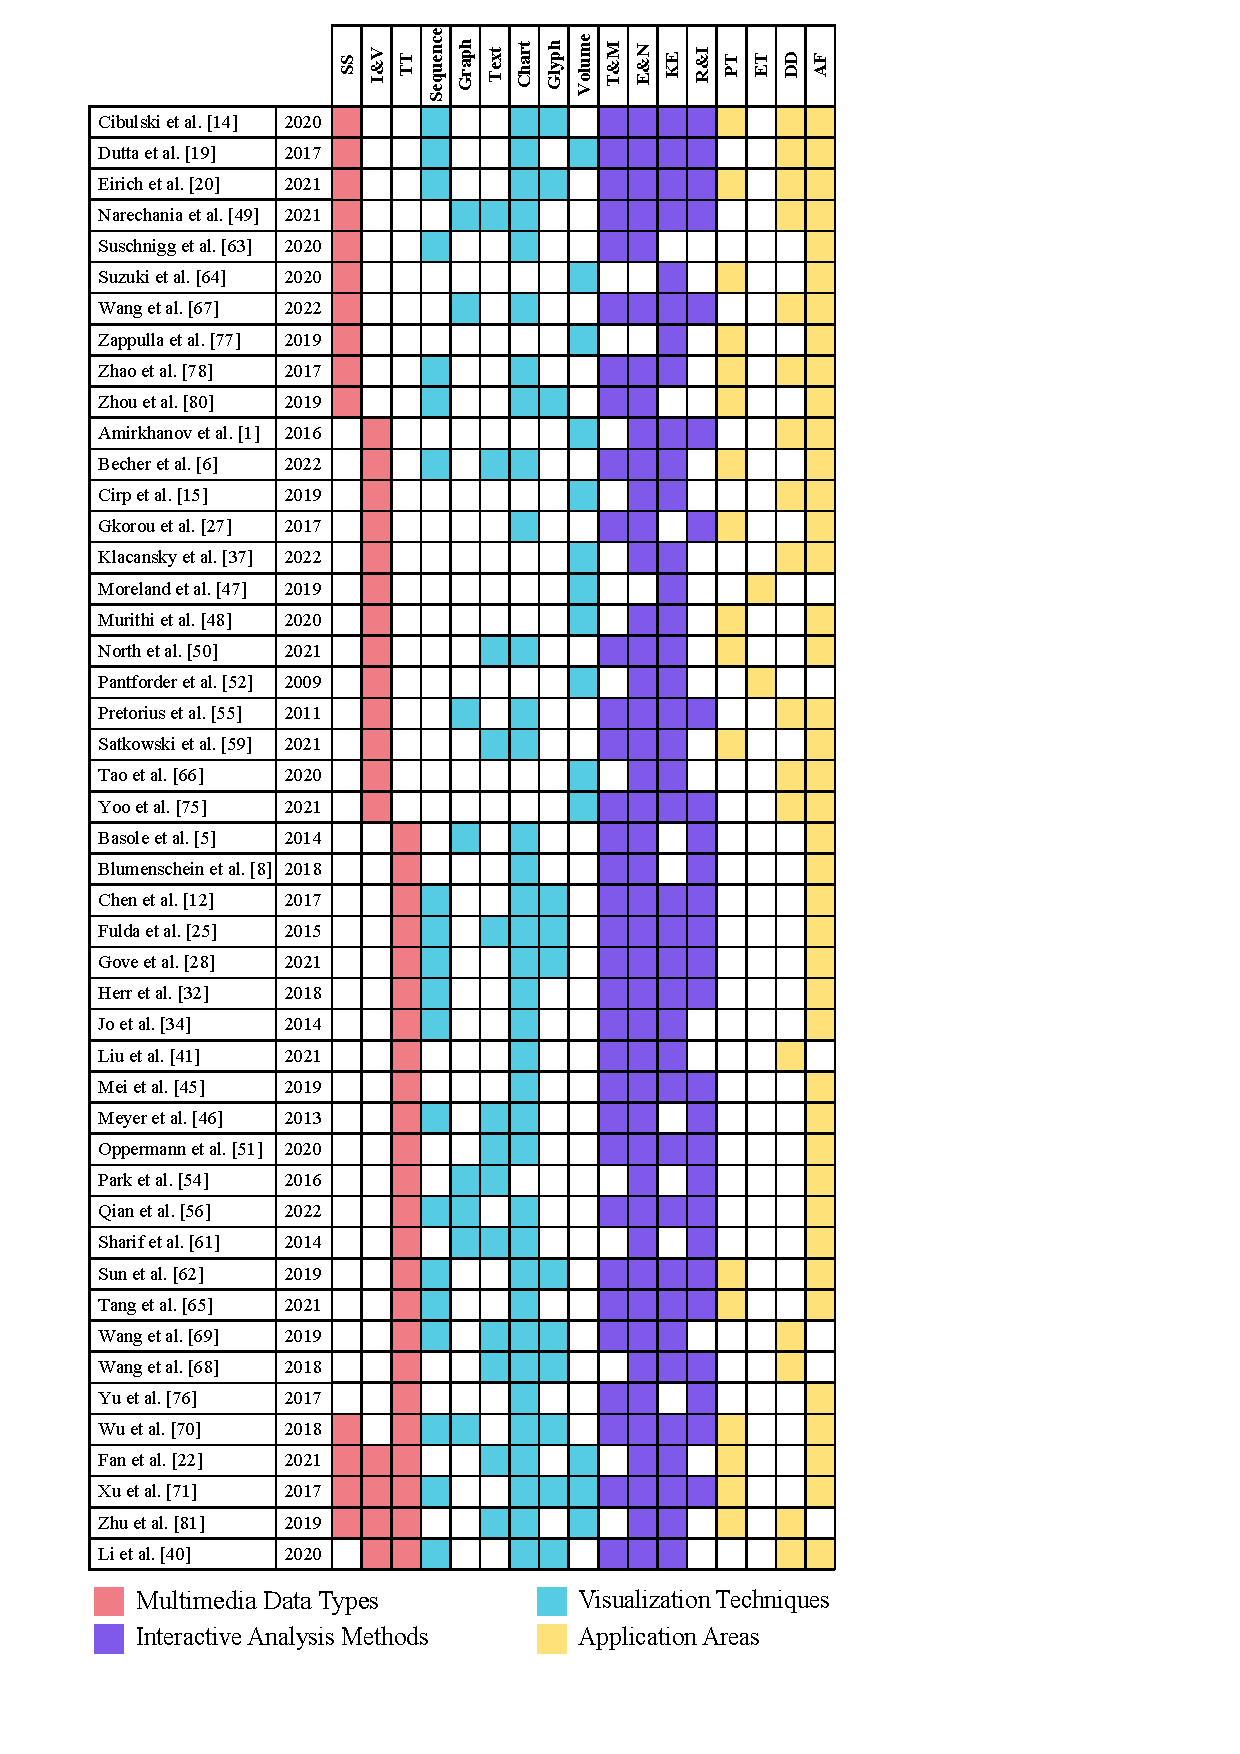
\includegraphics[width=0.48\textwidth]{Images/table.pdf}
	\caption{Categorization of the literature published in each section of this paper is based on manufacturing multimedia data types, visualization techniques, interaction analysis methods, and application areas.}
	\vspace{-1em}
	\label{table}
\end{figure}
 
%方法论
\subsection{Methodology}
%%为了阐明本调查的范围,我们阐明了我们工作中使用的三个术语:制造业、多媒体数据和可视化/可视分析。
To clarify the scope of this survey, we articulate three terms used in our work: manufacturing, multimedia data, and visualization/visual analytics.
%首先要说明是制造业是我们调查的领域。
First, it is important to note that manufacturing is the area we investigated.
%随着生产技术和社会需求的发展,制造业的门类不断完善。
With the development of production technology and social demand, the categories of manufacturing industry have been improved.
%现在中国国民经济行业分类中,制造业有31个大类,179个中类,609个小类。
Nowadays, there are 31 major categories, 179 medium categories and 609 small categories in China's national economic industry classification.
%我们主要对其中计算机技术普及程度较高的制造业类别进行调查。
We focus on those manufacturing categories which have a high degree of computer technology and automation.
%例如计算机制造、汽车整车制造、家用电力器具制造等。
For example, computer manufacturing, automobile manufacturing, household electric appliance manufacturing, etc.
%其次我们的分析对象是制造业全流程的多媒体数据,包括了结构化数据和非结构化数据。
Secondly, we analyze multimedia data from the whole process of manufacturing industry, including both structured and unstructured data. 
%传感器和计算机的使用,使得制造业中多媒体数据的收集越来越方便。
The usage of sensors and computers has made it increasingly convenient to collect multimedia data in manufacturing.
%因此,数据自身的实时性和数据间的关联性也有所增强。
Consequently, the real-time nature of data itself and the correlation between data have been enhanced.
%根据多媒体数据的类型进行针对性的快速细致的分析可以在制造业全流程的不同阶段做出及时的决策。
Targeted, rapid and detailed analysis based on the type of multimedia data can make timely decisions at different stages of the entire manufacturing process.
%这也是对制造业多媒体数据进行研究的内驱动力。
It is also the internal motivation for research on multimedia data in manufacturing.
%最后,我们我们关注的是运用在这些研究中的可视化与可视分析技术。
Finally, we are concerned with the visualization and visual analytics techniques used in these studies.
%可视化/可视分析技术因其直观性和有效性,被频繁应用在制造业多媒体数据的分析中。
Visualization/visual analysis techniques are frequently used in the analysis of multimedia data in the manufacturing industry because of their intuitiveness and effectiveness.
%我们希望调查在制造业多媒体数据分析中的可视化/可视分析技术,发现可视化研究社区感兴趣的应用领域,以及具体使用的可视化技术和交互分析方法。
We attempt to investigate visualization and visual analytics techniques of multimedia data in manufacturing to discover application areas of interest to the visualization research community, as well as visualization techniques and interactive analysis methods.

%我们对在可视化会议或者期刊上已发表的论文进行了关键词搜索。
We conducted a keyword search for papers that have been published in visualization conferences or journals to collect suitable literature.
%关键词的例子包括但不限于“制造业”,“工业”,“智能制造”,“制造业流程”,“工业4.0”。
Examples of keywords include but are not limited to "manufacturing", "industrial", "smart manufacturing", "manufacturing process ", "Industry 4.0".
%此外,我们的工作试图在其他高质量综述的基础上,探索制造业中可视化研究社区感兴趣的可视化技术、交互分析方法和应用领域。
Moreover, our work attempts to explore visualization techniques, interactive analysis methods, and application areas of interest to the visualization research community in manufacturing, building on other high-quality reviews.

%分类法
\subsection{Taxonomy}
%受第二节提到的高质量综述的启发,我们提出了一种新的基于数据类型的分类方法,对制造业多媒体数据的可视化与可视分析进行总结。
Inspired by the high-quality review mentioned in Section 2, we propose a novel taxonomy to summarize works related to the visualization and visual analysis of multimedia data in manufacturing.
%我们添加了最近发表的工作,并从可视化技术、交互式分析方法和应用领域进行详细讨论。
We add recently published works and discuss them in detail in terms of visualization techniques, interactive analysis methods and application areas.
%我们用不同的颜色对不同的分类维度进行编码:红色为多媒体数据类型、蓝色为可视化技术、紫色为交互式分析方法、黄色为应用领域。
We encode the different classification dimensions with different colors:
\raisebox{-0.4mm}{
\includegraphics[scale=0.25]{Images/red.png}} for multimedia data types, 
\raisebox{-0.4mm}{
\includegraphics[scale=0.25]{Images/blue.png}} for visualization techniques, 
\raisebox{-0.4mm}{
\includegraphics[scale=0.25]{Images/purple.png}} for interactive analysis methods, and 
\raisebox{-0.4mm}{
\includegraphics[scale=0.25]{Images/yellow.png}} for application areas.


%数据类型。从数据类型的角度可以将多媒体数据可以大致分为三大类:表格文本数据,传感信号数据、图像和视频数据。
\raisebox{-0.4mm}{
\includegraphics[scale=0.25]{Images/red.png}}
\textbf{Multimedia data types}. Multimedia data can be broadly classified into three main categories according to data types: \textit{Tabular text data} (TT), \textit{Signal sensing data} (SS), \textit{Image and video data} (IV).
%表格文本数据包含了以表格形式和文本形式存储的数据。制造业中有大量的数据是以表格形式存在的,例如销售记录、产品参数、生产日志等。用户投诉建议、产品描述、维修记录说明等则是以文本形式存储。
Tabular text data contains data stored in both tabular form and text form.
There is a large amount of data in the form of tabular forms, such as sales records, product parameters, production logs, etc. User complaints and suggestions, product descriptions, and maintenance record descriptions are stored in text form.
%信号传感数据包含了多种传感器收集到的数据,其中有声音传感器收集到的音频数据,有红外光学运动传感器收集到的动作数据,还有在物联网中的传感器收集到的轨迹数据。
Signal sensing data contains data collected by various sensors, including audio data collected by sound sensors, motion data collected by infrared optical motion sensors, and trajectory data collected by sensors in the IoT.
%图像视频数据中有一部分是由摄像机获取的真实数据,还有一部分是由数字仿真生成的。
Part of the image and video data is the real data acquired by cameras, and another part is generated by digital simulation.

%可视化技术。我们将应用在制造业多媒体数据的可视化技术分为顺序可视化、图可视化、文本可视化、图表可视化、字符可视化和体可视化。
\raisebox{-0.4mm}{
\includegraphics[scale=0.25]{Images/blue.png}}
\textbf{Visualization techniques}. We classify visualization techniques applied to multimedia data in manufacturing as \textit{sequence, graph, text, chart, glyph, and volume visualizations}. 
%序列可视化说明了数据具有的时间信息。序列可视化可以发现数据中异常情况,也可以探索数据的发展模式。通常,研究人员将时间作为单独的一个维度进行展示,例如规定一个坐标轴表示时间。与此相对应的可视化表现可以是折线图、流图。也可以对每个时间刻度上的数据属性进行更详细的展示,例如平行坐标系。
Sequence visualization illustrates the temporal information that the data has. Sequence visualization can identify anomalies in the data and explore patterns in the development. Generally, researchers present time as a separate dimension, for example by specifying a coordinate axis to represent time. The corresponding visual representation can be timeline visualization and flow visualization. More detailed presentation of data attributes on each time scale, such as parallel coordinate systems, is also available.
%图可视化是由点和边组成的网络结构。网络结构可以是有向的,也可以是无向的。常见的图可视化包括了节点链接图、树图、桑吉图。图可视化可以让用户发现数据之间的关联,例如数据的层级关系、属性联系、顺承关系。
Graph visualization is a network structure consisting of points and edges. The network structure can be directed or undirected. Typical  graph visualizations include node-link diagrams, trees, and Sankey diagrams. Graph visualization allows users to discover associations between data, such as hierarchical relationships, attribute associations, and codependencies.
%文本可视化主要关注是否在可视分析时引入文本数据。常见的文本可视化技术除了词云外,还会通过对文本内容进行高亮,以显示更多的上下文信息。
Text visualization focuses on whether to introduce text data in visual analysis. In addition to word clouds, text visualization can be visually enhanced by highlighting and also paired with other visualization techniques so as to show more contextual content, such as flow visualization.
%图表可视化主要是指借助了传统的可视化元素进行展示。例如散点图、柱状图、折线图、热力图和气泡图等。
Chart visualization mainly refers to the presentation with the help of traditional visualization elements. Typical chart visualizations are scatter, bar, line, heat and bubble charts, etc.
%字形可视化是指区别图表可视化,在可视化元素上进行了针对性的设计。
Distinguished from chart visualization, glyph visualization refers to the targeted design on visualization elements to produce a new visual representation.
%体可视化是指对物体进行三维地呈现。制造业中可以通过CT对物体进行扫描成像,也可以通过图像数据生成三维数字仿真。
Volume visualization can be described as the three-dimensional rendering of objects. In manufacturing, objects can be scanned and imaged by CT, or 3D digital simulations can be generated from image data.


%交互分析方法
\raisebox{-0.4mm}{
\includegraphics[scale=0.25]{Images/purple.png}}
\textbf{Interactive analysis methods}. 
%我们总结了在制造业多媒体数据可视化中常用的高层次交互分析方法,包括了追踪监控、探索导航、知识外化和细化识别。
We summarize the high-level interactive analysis methods~\cite{yi2007toward} which are commonly used in manufacturing multimedia data visualization, including \textit{Tracking \& Monitoring} (TM), \textit{Exploration \& Navigation} (EN), \textit{Knowledge Externalization} (KE), and \textit{Refinement \& Identification} (RI).
%追踪和监控:通过点击、悬停或者刷选对感兴趣的数据进行标记。
Tracking \& monitoring: mark data of interest by clicking, hovering or brushing.
%探索和导航:通过平移、缩放、下拉或滚动查看数据。  
Exploration \& navigation: review data by panning, zooming, drop-down or roll-up.
%知识外化:通过类似快照的方式对当前的可视化进行收集、保存和提取
Knowledge externalization: collect, save and extract current visualizations by taking snapshots.
%细化识别:通过已知的认证对数据进行标记。
Refinement \& identification: label data by known identities.
%研究人员和操作人员可以利用这四类交互分析方法完成制造业中的可视化分析任务。
Researchers and operators may use these four categories of interactive analysis methods to complete visualization and analysis tasks for manufacturing multimedia data.

%应用领域
\raisebox{-0.4mm}{
\includegraphics[scale=0.25]{Images/yellow.png}}
\textbf{Application areas}. 
%根据制造业实际生产需求,我们将制造业多媒体数据可视化与可视分析的应用领域分为四类:设计研发、工业生产、教育培训和分析反馈。
According to the actual production needs of the manufacturing industry, we classify the application areas of multimedia data visualization and visual analysis in manufacturing into four categories: \textit{Design \& Development} (DD), \textit{Industrial Production} (IP), \textit{Education \& Training} (ET), and \textit{Analysis \& Feedback} (AF).

%   表格文本数据
\section{Tabular Text Data}
%在本节,我们将针对制造业中的表格文本数据进行讨论。
In this section, we will discuss for tabular text data in manufacturing processes.
%表格文本数据是制造业中最常见的数据类型之一。本节讨论的表格文本数据包含了结构化数据、非结构化数据和半结构化数据。
Tabular text data is one of the most common types of data in manufacturing. The tabular text data discussed in this section contains structured data, unstructured data and semi-structured data.
%结构化数据是指可以使用关系型数据库表示和存储的,变现为二维形式的数据。每一行表示一个实体,每一列数据的属性是相同的。
Structured data is data that can be stored with relational databases and expressed in two-dimensional form. Each row represents an entity, and the attributes of each data column are the same.
%非结构数据是指没有一个预先定义好的数据模型或者方式来组织数据。文本数据就是典型的非结构化数据。
Unstructured data is data that is organized without predefined data models or methods. Text data is one of the typical unstructured data.
%半结构化数据是介于结构化数据和非结构化数据之间的数据。它并不符合关系型数据库或其他数据表的形式关联起来的数据模型结构,但包含相关标记,用来分隔的语义元素以及对记录和字段进行分层。因此,它也被称为自描述的结构,包括email、日志、XML文档和JSON文档。
Semi-structured data is data between structured and unstructured, which do not conform to the structure of the data model associated in the form of relational databases or other data tables, but contain associated tags, semantic elements for delimitation and hierarchy of records and fields. Therefore, it is also known as a self-describing structure that includes emails, log files, XML files and JSON files.
%制造业中的表格文本数据具有体量大、维度高、关系复杂的特点。可视化和可视分析的介入可以方便研究人员对表格文本数据进行更详细的分析。
Tabular text data in the manufacturing industry is large-scale, high-dimensional, and complex relational. The intervention of visualization and visual analysis can facilitate researchers to analyze the tabular text data with more details.

\begin{figure*}
	\centering
	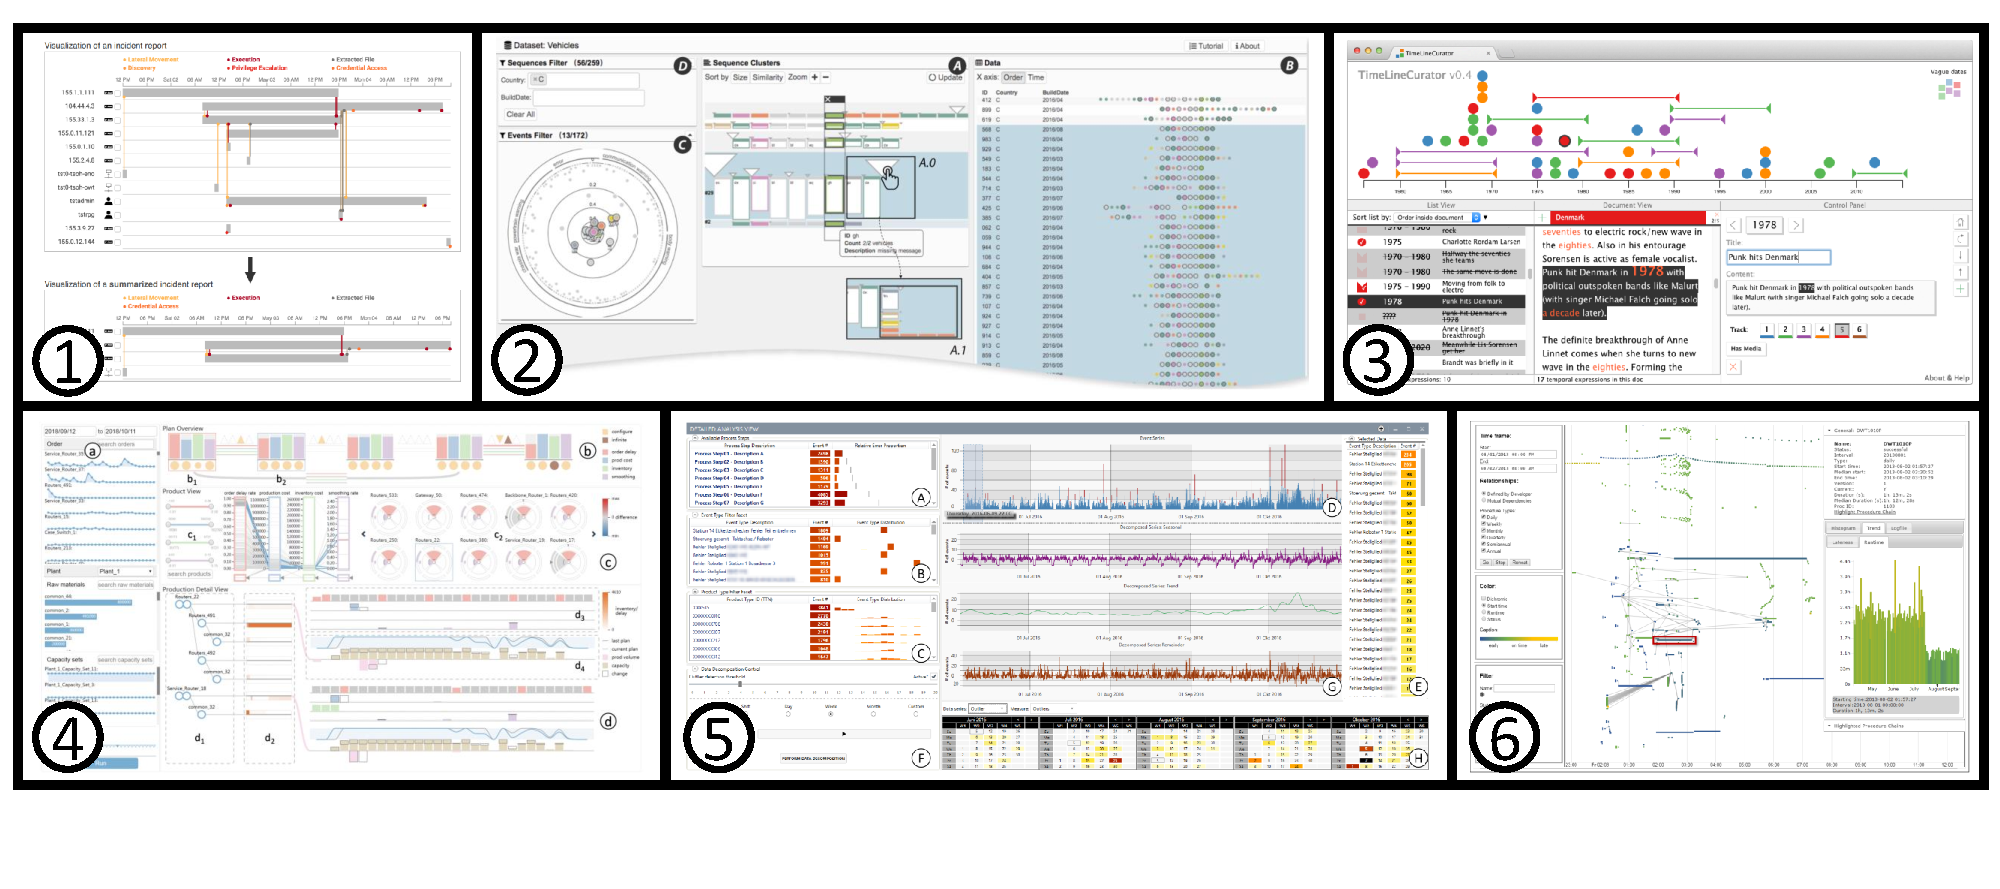
\includegraphics[width=\textwidth]{Images/tabular text data.pdf}
	\vspace{-4em}
	%表格文本数据对时间性的可视化。
	\caption{Visualization of temporality for tabular text data. (1) Visualization and summary of an incident report. (2) Visual analytics system for event sequence data exploration. (3) Display a timeline of Scandinavian pop music with TimeLineCurator. (4) Interface of PlanningVis which supports interactive exploration, comparison and optimization of production plans (5) Visual Analytics for Decomposing Temporal Event Series of Production Lines. (6) Visual monitoring of storage process runs.}
	\label{fig:tabulartextdata}
	\vspace{-1.5em}
\end{figure*}

%   可视化技术
\subsection{Visualization Techniques}
% 序列可视化可以表达表格文本数据的时间性。
Sequence visualization conveys temporality in tabular text data to users through a special form of visual communication. 
%依据时间的连续性,研究人员用线,弯的或者直的,代表时间。
Depending on the continuity of time, the researchers used lines, curved or straight, to represent time~\cite{bach2015time}.
%为了显示数据随时间的变化,研究人员在一维和二维形式的可视化中将时间作为一个维度。
To illustrate the variation of data over time, the researchers used time as a dimension in the visualization of both one and two dimensional forms.
%在一维的可视化形式中,数据直接在时间线上进行展示。在二维的可视化形式中,用直角坐标系中的X轴或者Y轴表示时间线。
In one-dimensional visualization, the data is presented directly on the timeline~\cite{chen2017sequence,fulda2015timelinecurator,Gove}. In two-dimensional visualization, the timeline is represented by x-axis or y-axis in rectangular coordinate~\cite{Friedl2021,herr2018visual,sun2019planningvis}.

%图可视化的研究应用于阐述数据中蕴涵的关系。park2016visual
Graph visualization is applied to explore the relationships involved in data~\cite{basole2014visual,Klammer2020,park2016visual,Qian2022,Sharif2014}.
%在Park等人设计的可视化分析系统中,网络图不仅集成了供应网络各种相关的观点和视角,还能突出供应网络的不同的结构。图可视化被Basole等人用来对供应网络风险进行可视分析,而RCDVis则用其交互式检测数据总的罕见类别。
In the visual analysis system designed by Park et al. the graph visualization not only integrates various relevant views and perspectives, but also highlights the different structures of a supply network~\cite{park2016visual}. Graph visualization was used by Basole et al.~\cite{basole2014visual} for visual analysis of supply network risk, while RCDVis~\cite{Qian2022} was used to interactively detect rare categories.

%图形可视化中,散点图可以显示离散数据的分布,平行坐标系可以显示多属性数据,折线图和直方图可以显示数据大小和变化趋势。
In chart visualization, scatter plots can illustrate the distribution of discrete data~\cite{Mei2019,Fellow2017}, parallel coordinates can display multi-attribute data~\cite{Fellow2017}, line and bar charts can show data volume and trend~\cite{sun2019planningvis,Oppermann}. 
%SMARTexplore用矩阵图和热力图展示高维数据。McNutt使用代数可视化对表格制图做了分析。
SMARTexplore presented high-dimensional data with matrix and heat maps~\cite{Blumenschein2018}. McNutt made an analysis of table cartograms with algebraic visualization design~\cite{McNutt2021}.

%字形可视化在其设计中会隐喻数据的一些属性融入。
Glyph visualization metaphorically incorporates some attributes of the data in its design~\cite{chen2017sequence,sun2019planningvis}. 
%PlanningVis利用基于时间轴的字形来表示各种生产计划及其差异的汇总信息。这个字形视图可以揭示配置变化的宏观影响,包括改进计划和模拟市场或工厂中的意外事件。
PlanningVis used timeline based glyphs to present summarized information of various production plans and their differences. By using this glyph view, you can reveal the macro impact of configuration changes, including improving the plan and simulating unexpected events in the market or factory.~\cite{sun2019planningvis}.
%chen等人用三角形符号编码事件插入的数量。用户双击原型中的三角形符号对它们进行详细分析。
Chen et al.~\cite{chen2017sequence} used triangle glyphs to encode the number of event insertions. Users can double-click on the triangle glyphs in the prototype to analyze them in detail.

\begin{figure}[pos=h]
	\centering
	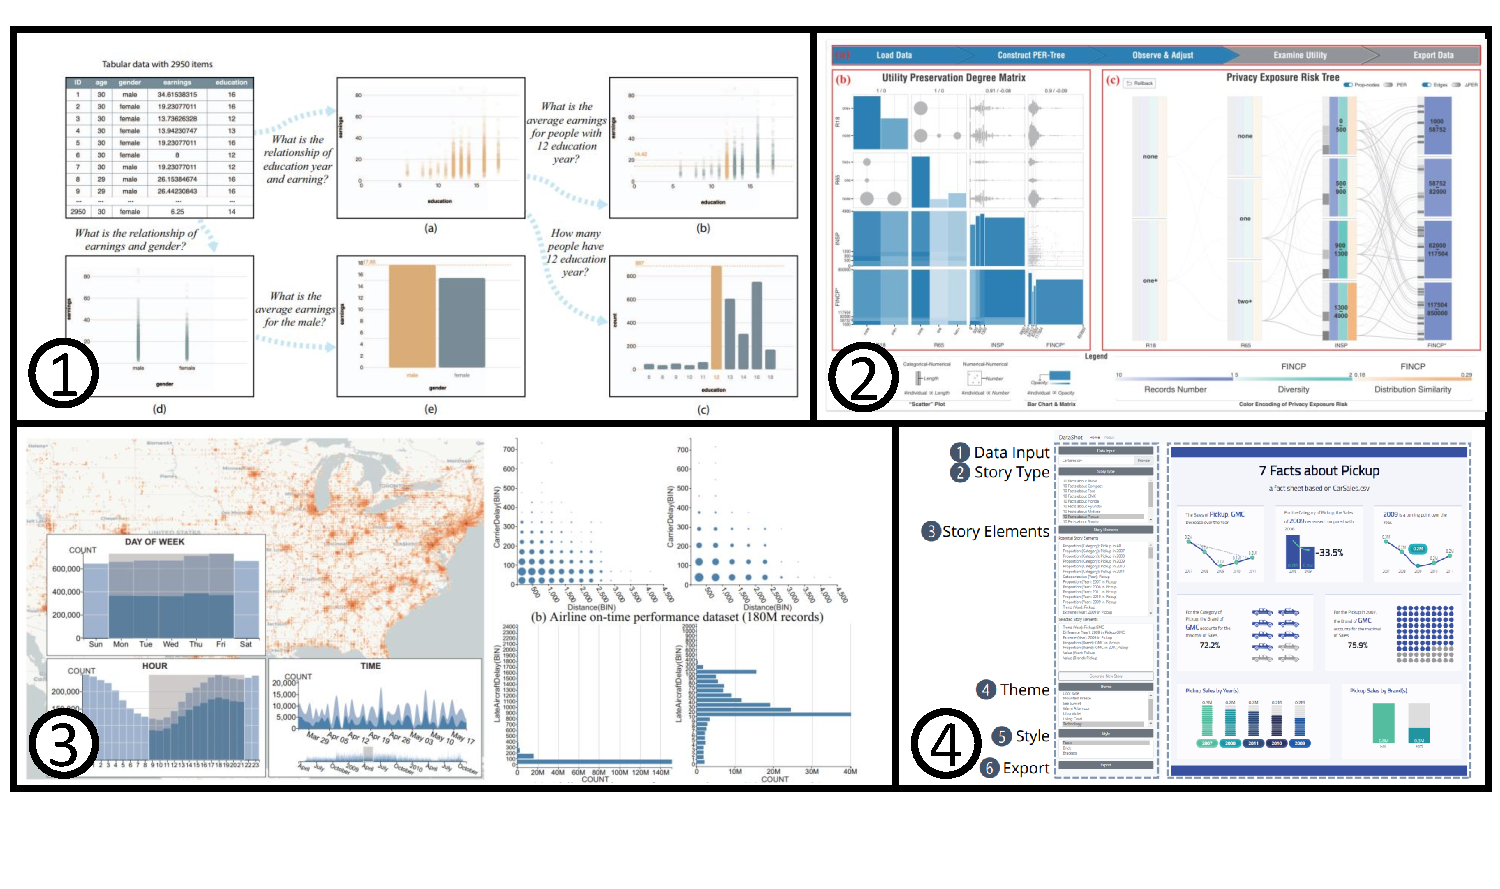
\includegraphics[width=0.49\textwidth]{Images/tabulartextdata2.pdf}
	\vspace{-3em}
	%图像和视频数据应用于缺陷检测的研究。
	\caption{Models and algorithms applied to tabular text data.}
	\label{fig:tabulartextdata2}
	\vspace{-1.5em}
\end{figure}

%   交互分析手段
\subsection{Interactive Analysis Methods}
%交互分析手段能减少表格文本数据体量大、维度高、关系复杂所带来的挑战。
Interactive analysis methods reduce the challenges posed by the large volume, high dimensionality and complex relationships of tabular text data.
%追踪和监控可以让用户在高度集成或者信息隐藏的可视化分析系统中追踪重要的信息。LiveGantt利用悬停的方式展示详细信息。Meyert等人通过框选显示存储过程的详细信息。
Tracking \& monitoring allows users to track important information in a highly integrated or information-hidden visual analytics system.
LiveGantt~\cite{Jo2014} displays detailed information via mouse hover. Meyer et al.~\cite{Meyer2013} displayed the details of the stored procedure by brushing the target node.
%探索和导航提供了用户改变可视化视图。PlanningVis利用选择列表的下拉和上滚选择目标数据集。
Exploration \& navigation provides users access to change visualization view. PlanningVis~\cite{sun2019planningvis} used drop-down and roll-up of list to select target dataset.
%DataShot从数据表中提取了大量有趣的数据,然后根据训练好的决策树将数据映射为可视化,并将其进行外部表达。
DataShot~\cite{wang2019datashot} extracted a large amount of interesting data from the data table, then mapped the data to visualizations based on a trained decision trees and expressed them externally.
%不同的交互式分析手段结合在可视化分析系统是常见的现象。
It is common for different interactive analysis methods to complement each other in visual analytics systems~\cite{Qian2022,sun2019planningvis,Fellow2017}.
%在RCDVis中,用户除了可以标注稀有分类的节点进行“细化识别”,同时可以对节点链接图进行平移和缩放进行“探索和导航”。
In RCDVis, users can not only label the nodes corresponding to rare categories for refinement \& identification, but also pan and zoom the node link map for exploration \& navigation.

%   应用领域
\subsection{Application Areas}
%制造业表格文本数据中记录的数据是多源的,其应用领域大多是“分析反馈”。
Tabular text data of manufacturing is multi-source and mainly applied for analysis \& feedback~\cite{Gove,Mei2019,sun2019planningvis,Wang2018}.
%RCDVis通过对图的交互式分析检测数据中的罕见类别。
RCDVis~\cite{Qian2022} detected rare categories among graph data  by interactive analysis.
%Gove提出了一种叙事摘要算法,对事件报告和网络日志进行叙事可视化,提高了报告精度。
Gove~\cite{Gove} proposed a narrative summary algorithm to visualize incident reports and network logs, and its compact representation earned positive reviews from analysts.
%在工业生产,合理安排制造计划是十分关键的,为此PlanningVis和LiveGantt展开了详细的研究。
In industrial production, properly organizing manufacturing schedules is crucial, and PlanningVis~\cite{sun2019planningvis} and LiveGantt~\cite{Jo2014} have conducted extensive work on this topic.
%在设计研发,工作主要集中在如何提高表格文本数据的展示效果,其中与算法相关的,也有与自动化生成相关的。
In design and development, collected articles focus on how to improve the presentation of tabular text data. Some of them are related to algorithms~\cite{Bartram2022,McNutt2021,Mei2019}, and some to automated generation~\cite{Liu2021,Wang}.

%   讨论
\subsection{Discussion}
%除了制造业外,其他领域也会产生表格文本数据。尽管数据来源不同,但一些可视化与可视分析方法是通用的。
In addition to manufacturing, other fields also generate tabular text data. Despite that data comes from different sources, some visualization and visual analysis methods are versatile.
%例如工厂生产计划与列车时刻表类似,基于内容的文本相似性推荐可以用在维修日志的记录和图书馆书本的管理。
For example, factory production schedules are similar to train schedules which require time series analysis. Content-based text similarity recommendation can be used for maintenance log recording and library book management.
%我们发现,随着机器学习和人工智能的发展,表格文本数据的自动可视化生成很有发展空间。
With the development of machine learning and artificial intelligence, we found that automatic visual generation of tabular text data is promising.
%还有关于如何高效地展示数据和可视化布局的挑战急需解决。
There are also challenges about how to present data and visualize layouts efficiently that need to be addressed urgently~\cite{Blumenschein2018,Mei2019}.

%   传感信号数据
\section{Signal Sensing Data}
%在本节,我们将针对制造业中传感信号数据进行讨论。
In this section, we will discuss for signal sensing data in manufacturing processes.
%在工业生产中,各式各样的传感器被用于采集机械设备,流水线和生产产品的信息。
A wide variety of sensors are used in manufacturing production to collect data from mechanical equipment, manufacturing lines, and manufactured products.
%这些传感器记录了设备的各种数据,如:温度,湿度,压力,流量,速度,位置等。
These sensors record various data of the equipment, such as: temperature, humidity, pressure, flow, speed, position, etc.
%视觉分析作为解释和解释复杂数据的重要技术,越来越多地应用于工业数据分析中。
Visual analytics is increasingly being used in industrial data analysis settings as a momentous technology for explaining and interpreting complex data.

\begin{figure*}
	\centering
	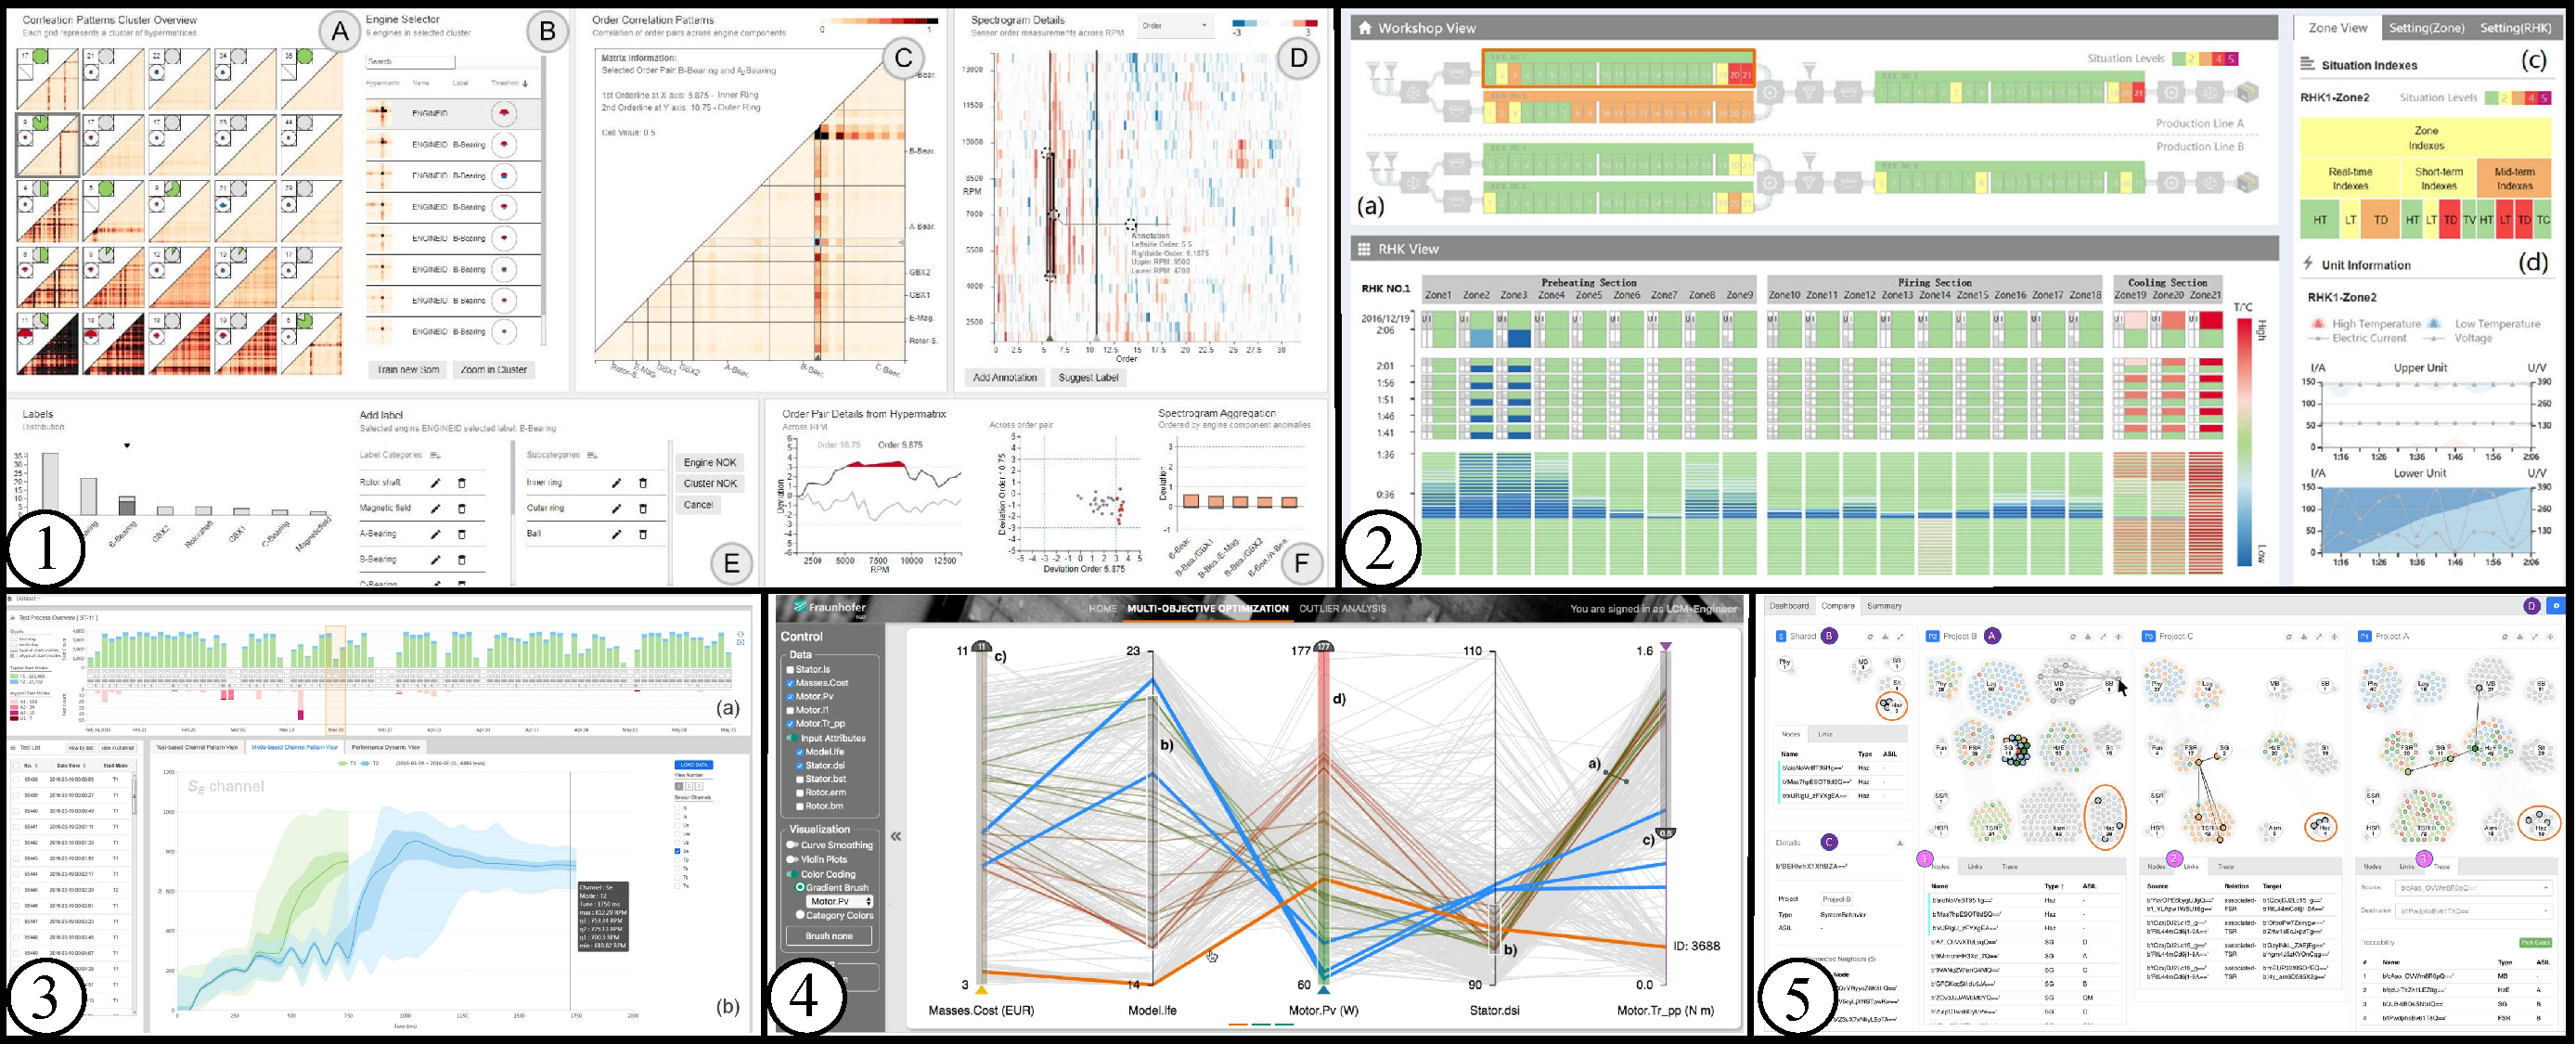
\includegraphics[width=\textwidth]{Images/signal data.pdf}
	\vspace{-1em}
	%表格文本数据对时间性的可视化。
	\caption{Visualization and anlysis for signal sensing data. (1) Visualizing and analyzing correlation patterns of	electrical engines. (2) Situation awareness and visual analytics for the routine monitoring and troubleshooting of Roller Hearth Kiln. (3) Visual analysis for understanding durability of automotive products. (4) Pareto front visualization for engineering design. (5) Visual data analysis of functional safety of vehicles.}
	\label{fig:signaldata}
	\vspace{-1.5em}
\end{figure*}


%   可视化技术
\subsection{Visualization Techniques}
%序列可视化在传感信号数据中非常普遍。
Sequence visualization is highly prevalent in sensing signal data.
%Zhao等人提出了一种利用大规模长期耐久性试验数据的可视化分析方法,来研究汽车起动机耐久性的关键因素。
Zhao et al. \cite{zhao2019visual} proposed a visual analysis method using large-scale and long-term durability test data to  investigate the key factor of the durability of automotive starters.
%基于不同传感器记录的发动机转速、发动机扭矩、温度、压力和废气测量数据,提出了一种灵活、可扩展的发动机异常检测可视化分析方法。
Based on engine speed, engine torque, temperatures, pressures and exhaust gas measures data recorded by varied sensors, Suschnigg et al. \cite{suschnigg2020exploration} presented a flexible and expandable visual analytics approach for anomaly detection on engine.
%Kagaya等人开发了一种技术,使用运动传感器来记录预防性维修期间工人动作的时序三维坐标数据,以便提取高质量维修工作的重要迹象。
Kagaya et al. \cite{Kagaya2017} developed a technique using a motion sensor to record time-series 3-D coordinate data of a worker's motions during preventative maintenance in order to extract important indications of high-quality maintenance work.

%图表可视化通常用于分析不同类型的信号传感数据,完成可视化分析任务。
Chart visualization is commonly employed to analyze different types of signal sensing data and complete visual analysis tasks.
%zhou等人设计了一个信息丰富的视觉分析系统,以实现复杂的关键制造设施辊道窑的常规监视和故障排除。
Zhou et al. \cite{Zhou2018} designed an informative visual analysis system to achieve the routine monitoring and troubleshooting of the complex key manufacturing facility Roller Hearth Kiln.
%Wang等人开发了带有节点链接图和详细数据视图的AFExplorer,以探索音频特征子集。
Wang et al. \cite{Wang2022} developed the AFExplorer with node-link diagram and detailed data view to explore the audio feature subset.
%IRVINE使用声学数据来检测和理解电气发动机制造中以前未知的错误。
IRVINE \cite{eirich2021irvine} used acoustic data to detect and understand previously unknown errors in the manufacturing of electrical engines.
% PAVED提供了一种交互式平行坐标可视化方法,以帮助工程师探索具有众多参数和标准的设计方案。
PAVED \cite{cibulski2020paved} provided an interactive parallel coordinates visualization to assist engineers to explore design alternatives, which are characterized by numerous parameters and criteria.
%SafetyLens是一个可视化的数据分析工具,结合了网络和集群探索技术,帮助工程师分析汽车功能安全数据集。
SafetyLens, \cite{narechania2020safetylens}a visual data analysis tool, which combined network and cluster exploration techniques to help engineers in analyzing automotive Functional Safety datasets.

%体可视化常被研发人员用来设计制造产品和仿真模拟。
Volume visualization is frequently utilized by developers to design products and perform simulations.
%Suzuki等人选择体积可视化来显示结构中的载荷路径,并将纤维与载荷路径的方向对齐。
Suzuki et al. \cite{Suzuki2020} chose volume visualization to display a load path in the composite material structure and aligned fiber with the direction of load path.
%Matthew等人介绍了一种处理来自温度传感器的高密度数据的方法,并使用三维可视化来显示连续钢坯铸造过程中模具区域的热流体流场。
Matthew et al. \cite{Zappulla2019} introduced a methodology for the processing of high-density data from temperature sensors and used 3D visualization of thermal fluid flow fields in mold region during continuous steel-slab casting.
%Huettenberger使用光学测量产生的数据,将汽车部件上的系统误差区域可视化,以实现自动检测。
Huettenberger et al. \cite{Huettenberger2015} used the data produced by optical measurements to visualize the areas of systematic errors on auto parts in order to achieve automatic detection.
%Dutta等人开发了基于GMM数据的可视化技术,使用表面渲染和不确定的等值线来检测跨音速喷气发动机失速的早期迹象。
Dutta et al. \cite{dutta2016situ} developed the tech of visualization of GMM based data using surface renderings and uncertain isocontours to detect the early signs of transonic jet engine stall.
%   交互分析手段
\subsection{Interactive Analysis Methods}
% 交互式分析方法使研究人员挖掘传感信号数据的隐藏模式和价值信息。
Interactive analysis methods assist researchers in uncovering hidden patterns and worthwhile information in signal sensing data.
%研究人员设计的原型系统提供了一套操作,帮助用户实现交互式数据探索。
The prototype systems \cite{eirich2021irvine, narechania2020safetylens, suschnigg2020exploration, zhao2019visual, Zhou2018} designed by researchers provide a set of operations to assist users achieve interactive data exploration. 
%跟踪和监控帮助用户进行流畅的数据探索。
Tracking \& monitoring assist users in carrying out fluent data exploration.
%zhao等人在许多视图和面板中提供交互。当用户在每个视图中移动或点击鼠标时,将显示详细信息。为进一步的观察和分析提供了多视图显示模式。
Zhao et al. \cite{zhao2019visual} and Zhou et al. \cite{Zhou2018} provided interaction in many views and panels. When users move or click the mouse in each view, detailed information will displayed. In addition, they provided a multiple-view display mode for further observation and analysis. 
%探索&导航为用户提供按需细节和视图更新。
Exploration \& navigation provide detail-on-demand and views update for users.
%PAVED通过鼠标光标的变换提供了对电机参数子集性能约束和偏好的选择。
PAVED \cite{cibulski2020paved} offered a selection on motor parameter subset performance constraints and preferences by a transformation of the mouse cursor.
%知识外化和细化识别被经常用于异常发现和态势监测方面。
Knowledge \& Externalization and Refinement \& Identification are commonly utilized in anomaly detection and situational monitoring.
IRVINE \cite{eirich2021irvine} combines interactive clustering and data labeling techniques, allowing users to analyze clusters of engines with similar signatures. Analysing signatures from engines acoustic data to detect and understand previously unknown errors.
%   应用领域
\subsection{Application Areas}
%信号传感数据来源众多,主要应用于设计开发、工业生产、分析反馈领域。
Signal sensing data come from numerous sources and are mainly applied to \textit{Design \& Development}, \textit{Industrial Production}, and \textit{Analysis \& Feedback}.
%这些工作应用光学,压力和温度传感器数据可视化制造材料和制造产品。其他工作致力于通过可视化技术分析多传感数据用于研究制造产品的耐久性,安全性,和异常状态。
In Design \& Development, these work \cite{Huettenberger2015, Suzuki2020, Zappulla2019} use optical, pressure and temperature sensor data to visualize manufacturing materials and manufactured products. Other work are devoted to the analysis of multi-sensor data through visualization techniques for the study of durability \cite{zhao2019visual}, safety \cite{narechania2020safetylens}, and abnormal states \cite{eirich2021irvine} of manufactured products.
% 在工业生产中,一些可视分析系统被设计用于工业生产态势监测,生产质量控制,生产产品检验。
In Industrial Production, several visual analytics systems are designed for industrial production situational monitoring \cite{Zhou2018}, production quality control \cite{Huettenberger2015} and manufacturing product inspection \cite{eirich2021irvine}.
%大多数研究工作都有分析反馈环节,比如:通过人机交互和专家合作方式分析参数集合用于改进电动机。
In Analysis \& Feedback, most of the research work have the analytical feedback component, e.g., the analysis of parameter sets for the improvement of electric motor design by means of human-computer interaction and expert collaboration \cite{cibulski2020paved}.


%   讨论
\subsection{Discussion}
%由于信号数据的多样性和复杂性,通用的可视分析方案和框架很难应用于制造产业的研发与生产过程。目前的可视化研究工作是针对某个具体的制造环节和制造产品的研发,比如: PAVED, IRVINE, SafetyLens等。这些可视分析系统的确帮助解决了一些实际工业生产制造和设计研发中的难题。但这些工作往往都需要专业的工程师一起协作,过高的专业性使可视化方案不再具有普适性。另外,在多传感器数据分析方面,如何利用好这些多元化数据去发现新的模式是值得我们去研究的。
Due to the diversity and complexity of signal data, generic visual analytics solutions and frameworks are difficult to apply to research and development and production processes in the manufacturing industry.
Current visualization research is focused on the development of a specific industrial segment and product, such as SafetyLens \cite{narechania2020safetylens}, PAVED \cite{cibulski2020paved}, IRVINE \cite{eirich2021irvine}, and so on. These visual analytics systems do help to solve some challenges in actual industrial manufacturing and design development. However, these efforts commonly require professional engineers to work together, and the excessive specialization makes the visualization solutions no longer universal. In addition, when it comes to multi-sensor data analysis, it is worthwhile to investigate how making good use of these diversified data to discover new patterns. 
%   图像视频数据
\section{Image \& Video Data}
%在本节,我们将针对制造业中图像视频数据进行讨论
In this section, we will discuss for image and video data in manufacturing processes.
%摄影摄像设备在制造业中的应用,产生了大量的图像视频数据。这些数据通常被用来监测工厂设备的运行情况、检测产品质量。
The application of photographic camera equipments in the manufacturing industry generate a large amount of image and video data, which are used to monitor the operation of equipment in factories and to check the quality of products.
%视频数据在按帧抽取后,也可以视为图像数据。因此,处理两种数据的方法在一定程度上是可以通用的。
Video data, when extracted by frame, can also be considered as image data. Therefore, the methods for handling both kinds of data can be common to some extent.
%以往对图象和视频的分析需要人的介入。这耗费了大量的人力,而且无法做到效率和准确率之间的平衡。
Previously, the analysis of images and videos required human intervention. It was labor-intensive and the balance between efficiency and accuracy could not be maintained.
%随着计算机计算能力和GPU性能的增强,对图像和视频数据的分析研究变得更为方便,成为制造业多媒体数据中的新兴研究方向。
With the enhancement of computer computing power and GPU performance, the analysis and research of image and video data have become more convenient and become an emerging research direction in manufacturing multimedia data.
%同时,近些年人工智能和机器学习的崛起,使得即高效有准确的处理图象和视频数据成为可能。
At the same time, the rise of artificial intelligence and machine learning in recent years has made it possible to process image and video data efficiently and accurately.
%而虚拟现实和增强现实的发展,使得分析数据从二维扩展到三维,同时增加了新的可视化展示和交互分析方法。
And the development of virtual reality and augmented reality has expanded the analysis of data from two-dimensional to three-dimensional, while adding new visual displays and interactive analysis methods.

\begin{figure}[pos=h]
	\centering
	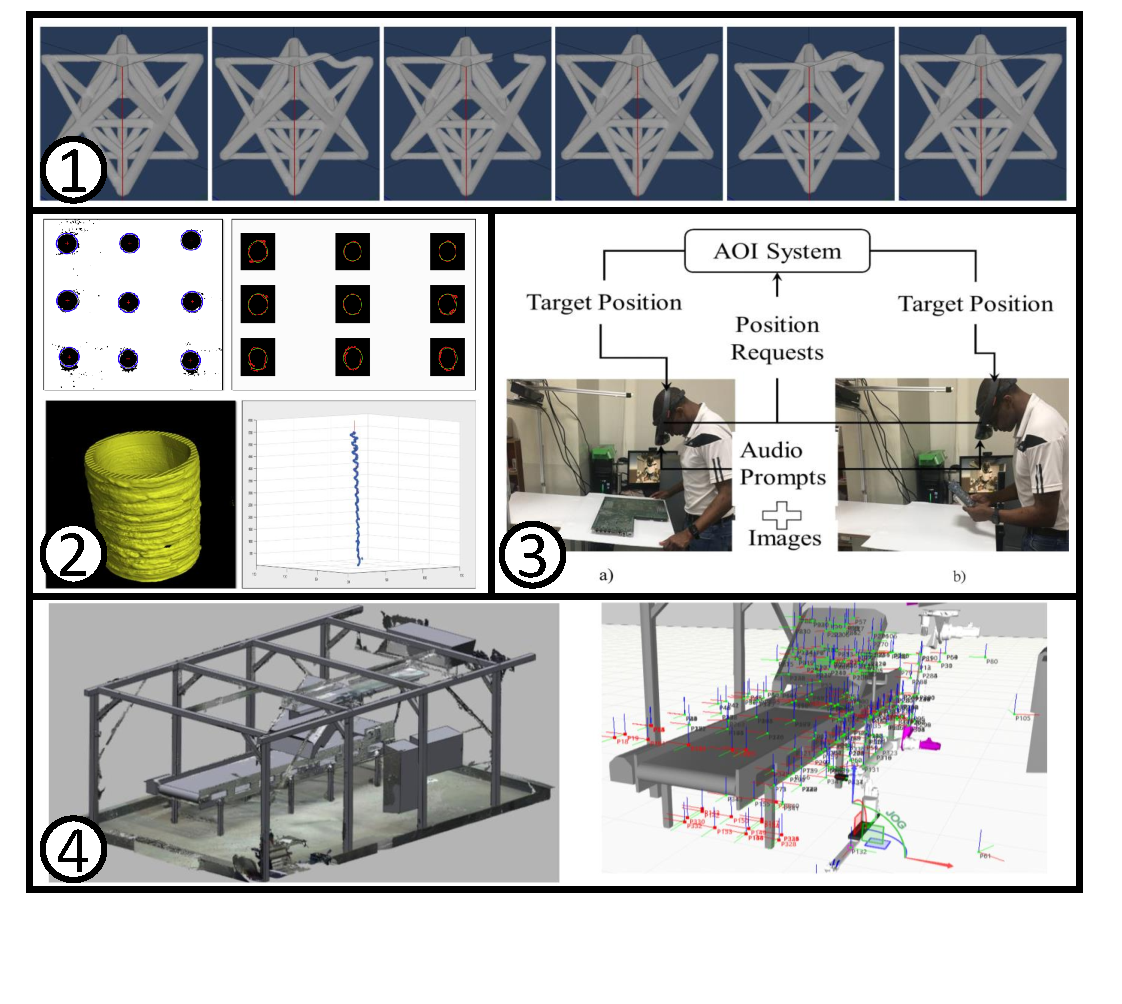
\includegraphics[width=0.48\textwidth]{Images/imageandvideo.pdf}
	\vspace{-4em}
	%图像和视频数据应用于缺陷检测的研究。
	\caption{Research on the application of image and video data for defect detection.(1) Volume visualization of the physical structure of additively manufactured parts, including one normal case (far left) and five abnormal cases. (2) Detection of the machining accuracy of PCB holes. (3) Markerless cooperative augmented reality-based intelligent manufacturing review system. (4) Check the equipment installation with 3D scanning.}
	\label{fig:imageandvideo}
	\vspace{-1.5em}
\end{figure}

%   可视化技术
\subsection{Visualization Techniques}
%为了方便分类和参数关系的展示,图经常在对图像和视频数据进行分析的相关研究中被看到。
Graph visualization is often seen in relevant researches for the analysis of image and video data in order to facilitate the classification and the presentation of parameter relationships.
%Pretorius等人提出了一种基于参数采样和交互式视觉探索的优化参数的范式变化。他们设计了一个叫做Paramorama的原型。其中输入参数和相应输出之间的关系就是用来树(有向无环图)来展示的。
Pretorius et al.~\cite{Pretorius2011} proposed a paradigm shift for optimizing parameters based on parameter sampling and interactive visual exploration. They designed a prototype called Paramorama. Where the relationship between the input parameters and the corresponding outputs was presented using a tree (directed acyclic graph).
%CommunityDiff中在节点-链接图的基础上增加了额外的约束,从而对相同社区的节点进行分类,同时保持节点之间的联系。
Additional constraints were added to the node-link graph in \textit{CommunityDiff}~\cite{Emelyanova} so that nodes classified as the same community are restricted to the same rectangle, while maintaining connections between nodes.
%在Locomotion Vault,一个可视化工具和数据库,中也用了节点-链接图来表示不同技术之间的相似度。
Node-link graphs are also used in \textit{Locomotion Vault}~\cite{Luca2021}, a visualization tool and a database of over 100 techniques that were proposed by researchers and practitioners in the academia and industry, to represent the similarity between different technologies.

%图表可视化在图像和视频分析中也较为常见。在Gkorou等人的工作中,将用于监控和诊断大容量半导体制造的最相关因素进行可视化并进行排名,其中运用了散点图、热力图和盒须图。
Chart visualization is one of the common visualization techniques used in image and video data analysis. In the work of Gkorou et al~\cite{Gkorou2017}. the most relevant factors for monitoring and diagnosing high volume semiconductor manufacturing were visualized and ranked, where scatter plot, heatmap and boxplot were utilized.
%Locomotion Vault中使用了柱状图来展示每一年中技术的数量。
Bar chart was used in \textit{Locomotion Vault} to show the number of technologies in each year.

%利用三维扫描或者数字仿真的技术,我们可以对产品和工业设备进行体可视化。
Volume visualization of products and industrial equipments can be performed by means of 3D scanning or digital simulation techniques.
%Amirkhanov等人利用4DCT数据对玻璃纤维增强聚合物进行数字建模,从而发现其缺陷。
Amirkhanov et al.~\cite{amirkhanov2016visual} used 4DCT data for numerical modeling of glass fiber reinforced polymers to find defects.
%Cirp等人通过3D扫描产生的3D空间数据进行模拟,从而对制造系统和原型设计进行可视化支持。
Cirp et al.~\cite{Cirp2019} simulated the 3D spatial data generated by 3D scanning to provide visualization support for designing manufacturing systems and prototypes.
%Tao等人基于X射线显微CT对PCB孔进行三维表面扫描,对加工精度进行检测。
Tao et al.~\cite{tao2020machining} performed 3D surface scanning of PCB holes based on X-ray micro-CT to check the machining accuracy.
%Design by Dragging 引入了一种新的方法,以尽可能直接的设计与模拟。

%   交互分析手段 
\subsection{Interactive Analysis Methods}
%交互分析手段可以让分析人员更好的对图像和视频数据进行追踪监控和分析研究,从而发掘数据中更深层的知识,并将反映出的知识反馈到实际工业生产活动中。
Interactive analytics methods allow researchers to better analyze image and video data to uncover deeper knowledge. 
% 追踪监控允许用户对特定的对象进行分析研究。
Tracking \& monitoring allow analysts to perform analytical research on target objects. 
%在Paramorama原型中,用户可以选择感兴趣的输入参数,然后追踪其与输出结果之间的关系。
In Paramorama prototype~\cite{Pretorius2011}, users can select the input parameters of interest and then trace their relationship with the output results.
% 探索导航通过对界面的平移和缩放,组织结构的展开和折叠,对图像参数之间的影响进行分析。
Exploration \& navigation analyze the impact between image parameters by panning and zooming the interface, expanding and collapsing the organizational structure.
%CommunityDiff中的利用树状图显示不同集合输出之间关系和比例。
CommunityDiff~\cite{Datta2018} used tree diagrams to show the relationships and proportions between the different collection outputs.
% 知识外化为研究人员外化当前可视化内容提供了一种途径。 
Knowledge externalization provides a way for researchers to externalize the content of current visualizations. 
%Satkowski等人以工业3D场景为背景,从主观感知和客观测量分析了视觉背景对增强现实的影响。
Satkowski et al~\cite{Satkowski2021}. analyzed the impact of visual context on augmented reality in terms of subjective perception and objective measurements using industrial 3D scenes as a background.
% 细化识别方便用户依据已知的身份对数据进行标记。
Refinement \& identification facilitate analysts to label data based on known identities.
%用户标记高质量和低质量的结果,对搜索结果进行优化。
Analysts label high and low quality results and optimize the search results in Paramorama prototype~\cite{Pretorius2011} .  

\begin{figure*}
	\centering
	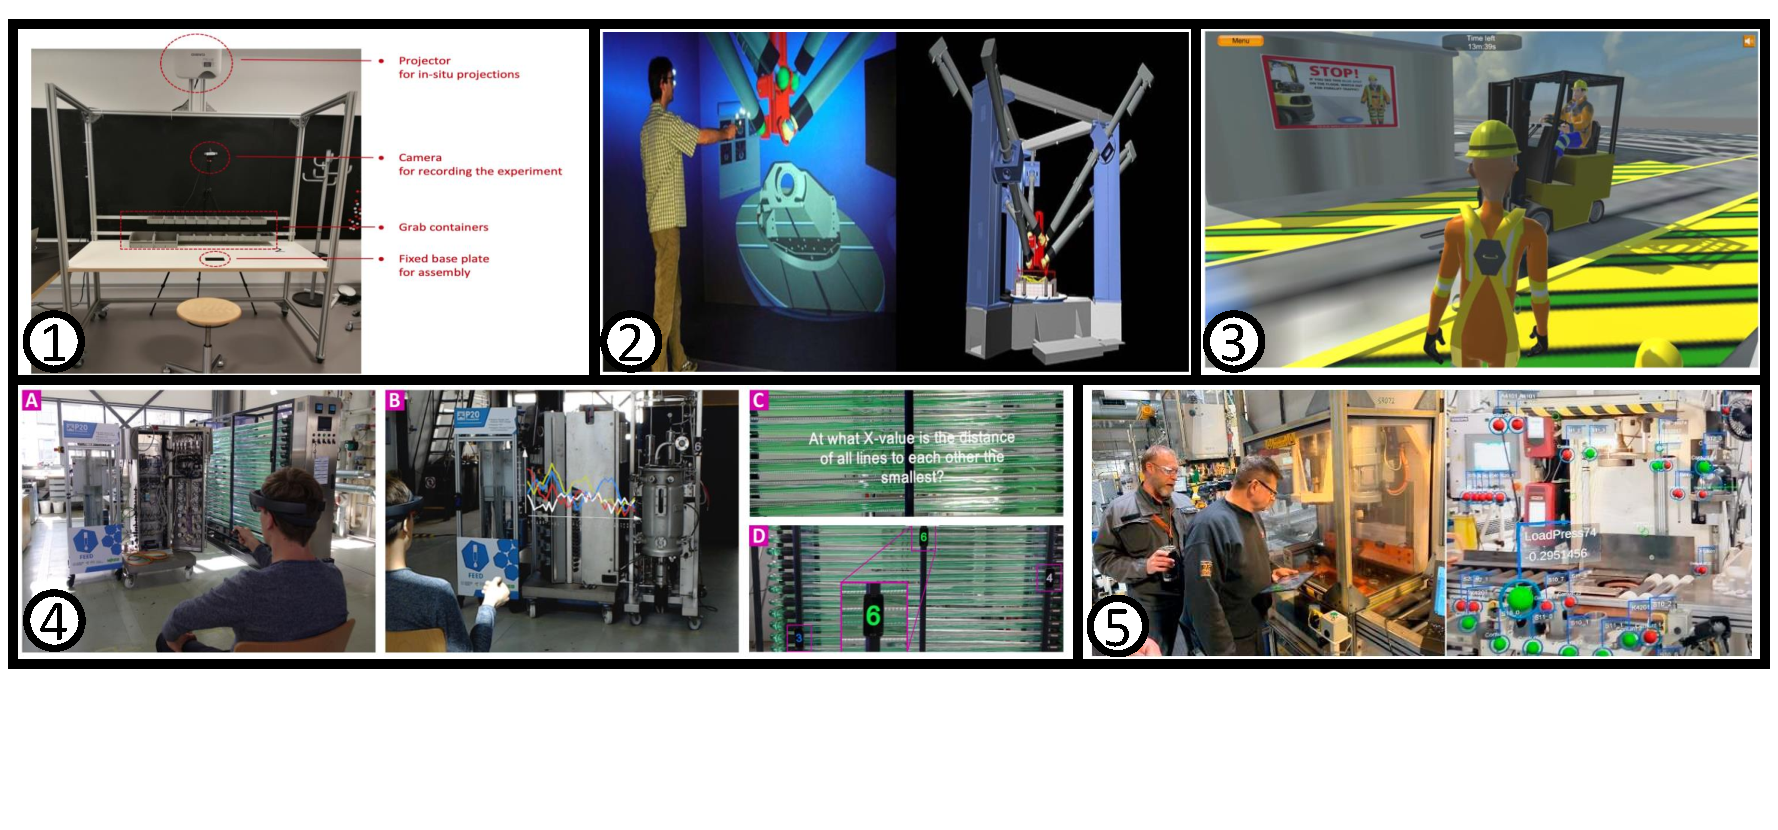
\includegraphics[width=\textwidth]{Images/imageandvideo2.pdf}
	\vspace{-5.5em}
	%增强现实和虚拟现实在制造业中的应用。
	\caption{Augmented reality and virtual reality in manufacturing. (1) Assisted industrial assembly training with a projection-based AR system. (2) Virtual reality applications in manufacturing systems. (3) Interactive simulator for steel industry safety training. (4) Augmented reality that uses the real factory environment as a background to display equipment information. (5) Final demonstration and use of the industrial internet of things (IIoT) based augmented reality for factory data collection and visualization by Volvo technicians.}
	\label{fig:imageandvideo2}
	\vspace{-2em}
\end{figure*}

%   应用领域
\subsection{Application Areas}
% 图像和视频数据贯穿了整个制造业流程。将虚拟现实和增强现实技术与图像和视频数据相结合,促进了可视化和可视分析在工业生产中的应用。
Image and video data exist throughout the manufacturing process. The application of visualization in industrial production is facilitated by integrating VR and AR technologies with image and video data~\cite{hamid2014virtual,Satkowski2021}. 
% 在分析反馈中,通过对图像和视频数据的可视分析,研究人员发现产品缺陷,验证加工工艺,检查设备安装。
In analysis \& feedback, researchers identify product defects, verify machining processes and check equipment installations through visual analysis of image and video data~\cite{Cirp2019,Murithi2020,tao2020machining}. 
%通过将用于监控和指导的AR头戴设备与用于更详细数据分析的便携式平板设备相结合,使现场操作人员能够及时对重大错误事件做出反应,并调查事件的历史,已确定因果关系。
By combining an AR headset for monitoring and guidance with a portable tablet device for more detailed data analysis, field operators are able to respond to major error events in a timely manner and investigate the history of the event to identify causality~\cite{Becher2022,Murithi2020,North2021,Satkowski2021}.
% 在设计研发中,研究人员会将分析和反馈中的不足之处进行总结,探究其产生原因,然后对产品进行完善。
In design \& development, researchers will summarize the shortcomings in analysis \& feedback, explore the reasons, and then improve the product~\cite{Townsend2022}.
% 在教育培训中,为了减少成本,增加趣味性,方便展开职工培训,研究人员根据生产数据和行业安全手册开发了特定行业的安全培训互动模拟器。同时,也有研究人员对增强现实在人员装配培训的应用进行了论证。
In education \& training, to reduce costs, increase interest and facilitate the roll-out of employee training, researchers developed industry-specific interactive safety training simulators based on production data and industry safety manuals~\cite{Moreland2019,Pantforder2009}. Meanwhile, some researchers have also discussed whether the usage of AR in personnel assembly training is justified~\cite{buttner2020augmented}.


%   讨论
\subsection{Discussion}
%早期图像和视频数据的研究集中在二维的图像数据,这可能是受限于计算机性能和可视化方式。一个值得注意的趋势是,AR和VR的使用越来越多。
Early studies of image and video data focused on 2D data, which may be limited by computer performance and visualization methods. A notable trend is the increasing use of AR and VR. 
%AR和VR设备相较于屏幕,拥有更强的交互性。以实际工厂为背景显示数据的AR,让操作员在巡视时可以直观的看到设备的运行数据。同样的,操作员可以通过AR设备在被检测的产品上显示其可能存在的缺陷。员工借助VR设备可以将虚拟环境中掌握生产流程、熟悉生产环境,提高了培训员工的效率和安全性。未来会有更多基于AR和VR设备的研究,包括展示高效展示更多的信息以及设备的拓展应用。
AR and VR devices have a more interactive nature than screens. Operators wear AR devices with actual production scenes as the background during their inspections, allowing them to visualize the operating data of the equipment~\cite{Satkowski2021}. Similarly, the operator can use the AR device to display possible defects on the product being inspected~\cite{Murithi2020}. With VR equipments, employees can master the production process and get familiar with the production environment virtually, which improves the efficiency and safety of training~\cite{hamid2014virtual}. In the future, there will be more research based on AR and VR devices, including demonstrating efficient display of more information and expanded applications of the devices.
%同时,数据维度也逐渐从二维扩展到三维。相较于平面,立体能够传达更多的信息。比如材料的物理结构信息,设备在立体空间中的位置关系等。为此,我们希望体可视化技术可以更多地应用在制造业中。
At the same time, the data dimension has been extended from 2D to 3D. Compared to two dimensions, three dimensions can convey more information. For example, the physical structure of the material and the position of the device in the 3D space. To this end, we hope that volume visualization technologies would be more widely used in manufacturing.

%  多种多媒体数据合作
\section{Multiple Multimedia Data Collaboration}
%在本节,我们将针对制造业流程中的多种多媒体数据合作的应用进行讨论。
In this section, we will discuss multiple multimedia data collaborations in manufacturing processes.
%总所周知,产品设计的数据一般是图象视频数据,而用户意见反馈的数据为表格文本数据,这两种多媒体数据类型是不同的。产品设计需要用户的意见反馈作为依据进行迭代更新。我们将此称为多种多媒体数据合作。
As we all know, product design data is generally image and video data, while user feedback data is tabular text data, these two types of multimedia data are different. Product design requires user feedback as the basis for iterative updates, and we refer to similar cases as multiple multimedia data collaboration.
%随着数字孪生概念的提出与实践,促进了多种多媒体数据的合作。
With the introduction and practice of the \textit{Digital Twin} (DT) concept, the collaboration of multiple multimedia data is promoted.
%可视化与可视分析作为一种工具,可以帮助研究人员减少数据来源多和数据类型不一致带来的分析负担。
Visualization and visual analytics as a tool can help researchers reduce the analytical burden associated with multiple data sources and inconsistent data types.
%同时在分析时增加交互功能,可以帮助研究人员更好的发觉数据之间的联系,从而做出更好的决策。
Moreover, adding some interactive functions can help researchers discover connections between data to make better decisions.
%我们选取几个常见的多媒体数据合作案例讲解可视化与可视分析在其中的作用。
We choose several multimedia data collaboration cases to explain the role of visualization and visual analytics.

%数字孪生
\subsection{Digital Twin}
%数字孪生是指通过集成物理反馈数据,并辅以人工智能、机器学习和软件分析,在信息化平台内建立一个数字化模拟。


% 总结和机会
\section{Conclusion And Opportunities}

\bibliographystyle{cas-model2-names}
\bibliography{multimedia}

\end{document}
